\documentclass[runningheads]{llncs}

\usepackage[utf8]{inputenc}
\usepackage{graphicx}
\usepackage{todonotes}
\usepackage{multirow}
\usepackage{array,booktabs,tabularx,ragged2e,caption}
\newcolumntype{M}[1]{>{\centering\arraybackslash}m{#1}}
\newcolumntype{C}[1]{>{\Centering}m{#1}}
\renewcommand\tabularxcolumn[1]{C{#1}}

\newcommand{\myblue}[1]{{\color{blue}{#1}}}
\newcommand{\myred}[1]{{\color{red}{#1}}}
\newcommand{\mygreen}[1]{{\color{ForestGreen}{#1}}}

\usepackage{multicol,lipsum}


\title{DICE @ Rich Context Competition 2018 -- Combining Embeddings and Conditional Random Fields for Research Dataset, Field and Method Recognition and Linking}
\titlerunning{DICE @ Rich Context Competition 2018}
\author{Rricha Jalota \and Nikit Srivastava \and Daniel Vollmers \and René Speck \and Michael R\"oder \and Ricardo Usbeck\orcidID{0000-0002-0191-7211} \and Axel-Cyrille {Ngonga Ngomo}}
\authorrunning{Jalota et al.}


\institute{
Data Science Group, Paderborn University, Germany\\
\email{firstname.lastname@uni-paderborn.de}
}

\begin{document}
%\lipsum[1]
\maketitle

\begin{abstract}
    The steadily increasing number of publications available to researchers makes it difficult to keep track of the state of the art. In particular, tracking the datasets used, topics addressed, experiments performed and results achieved by peers becomes increasingly tedious. Current academic search engines %such as Google Scholar, %\footnote{https://scholar.google.de}, Semantic Scholar, etc. 
    render a limited number of entries pertaining to this information. However, having this knowledge would be beneficial for researchers to become acquainted with all results and baselines relevant to the problems they aim to address. With our participation in NYU Coleridge Initiative’s Rich Context Competition, we aimed to provide approaches to automate the discovery of datasets, research fields and methods used in publications in the domain of Social Sciences. We trained an Entity Extraction model based on Conditional Random Fields and combined it with the results from a Simple Dataset Mention Search to detect datasets in an article.  For the identification of Fields and Methods, we used word embeddings. In this paper, we present how our approaches performed, their limitations, some of the challenges we encountered and our future agenda. 
\end{abstract}

\section{Introduction}
\subsection{Rich Context Competition}
The goal of the Rich Context Competition\footnote{\url{https://coleridgeinitiative.org/richcontextcompetition}}, organized by the New York University under their Coleridge Initiative, was to automate the discovery of research datasets, associated research methods and fields in research publications belonging to the domain of Social Sciences. It was carried out in two phases. 
In the first phase (Phase-1), we were provided with a list of datasets along with their metadata (dataset vocabulary), a training corpus of 5000 publications containing publication metadata (2500 of them were labeled) and an additional dev fold of 100 publications. Apart from this, we were also given Social Science Methods and Fields vocabularies by SAGE Publications\footnote{\url{https://uk.sagepub.com/en-gb/eur/home}}. To carry out Phase-1 evaluation, a separate corpus of 5000 labeled publications was held back.
%\todo[inline]{write about output files}

In the second phase (Phase-2), in addition to the Phase-1 data for training, we were provided with the Phase-1 holdout set consisting of 5000 labeled publications and an additional corpus of 5000 unlabeled publications. The evaluation of the second phase was carried out by the organizers on another corpus that contained 5000 unlabeled publications. Note that the labeled data in both the phases was for Dataset Detection only. There was no ground truth for Research Methods and Fields. 
%Note that, the labeled data in both the phases was for Dataset Detection only. There was no ground truth for Research Methods and Fields. 

\subsection{Project Architecture}

\begin{figure}[!htb]
    \centering
    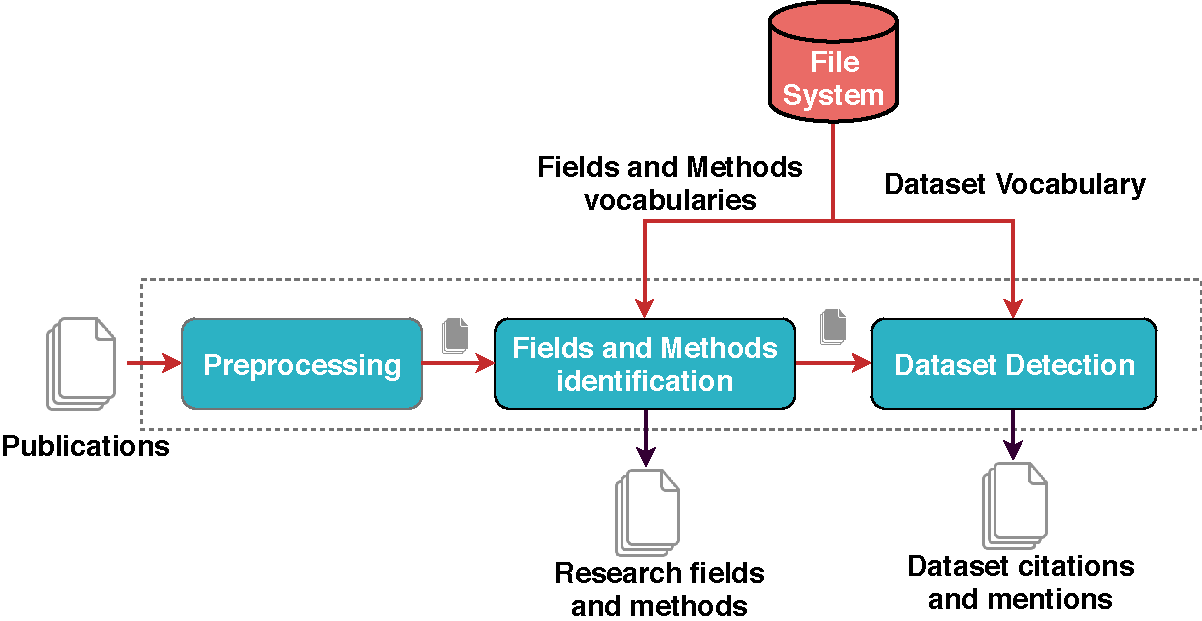
\includegraphics[width=0.99\textwidth]{images/flowchart_paper.pdf}
   %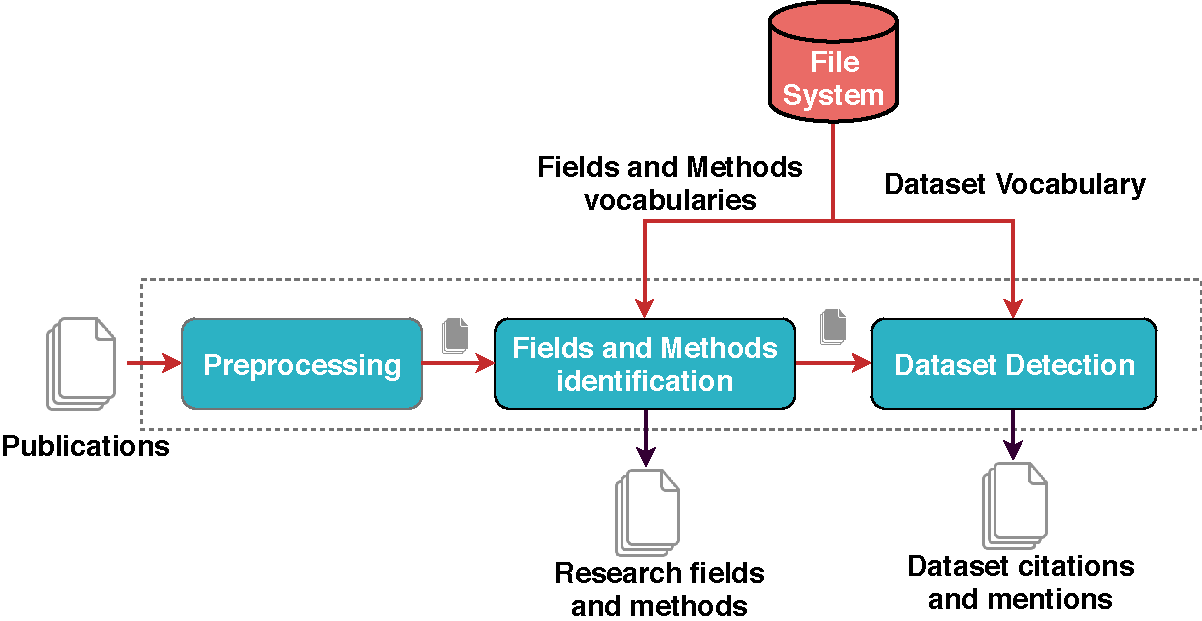
\includegraphics[scale=0.46]{images/flowchart_paper.pdf}
    \caption{Data Flow Pipeline (Red lines depict the flow of given and generated files between components whereas black lines represent the generation of final output files)}
    % \scriptsize{}
    \label{fig:flowchart}
\end{figure}

Our pipeline (shown in Fig. \ref{fig:flowchart}) consisted of three main components: 1) Preprocessing, 2) Fields and Methods Identification and 3) Dataset Extraction. The Preprocessing module read the text from publications and generated some additional files (see Section~\ref{preprocess} for details). These files along with the given Fields and Methods vocabularies were used to infer Research Fields and Methods from the publications. Then, the information regarding fields was passed onto the Dataset Detection module and using the Dataset Vocabulary, it identified Dataset Citations and Mentions. The following sections provide a detailed overview of each of these components. 

\section{Preprocessing} \label{preprocess}

The publications were provided to us in two formats: PDF and text. %the form of both PDF and text. 
For Phase-1, we used the given text files, however during Phase-2, we came across many articles in the training files that had not been properly converted to text and contained mostly  non-ASCII characters. In order to work with such articles, we relied on the open source tool \texttt{pdf2text} from \texttt{poppler suite}\footnote{\label{poppler}\url{https://manpages.debian.org/testing/poppler-utils}} to extract text from PDFs. \\

\smallskip

Once we had the text files, we followed the rule-based approach as proposed %\todo[inline]{did you omit a word after 'rule-based' or should it rather say 'proposal'}
in~\cite{DBLP:journals/ploscb/WestergaardSTJB18} for pre-processing. The following series of operations based mostly on regular expressions were performed:
\begin{itemize}
    \item Words split by hyphens were de-hyphenated %\todo[inline]{should you be more specific than 'handled'? Unclear what that means};
    \item Irrelevant data was removed (i.e., equations, tables, acknowledgment, references);
    \item \raggedright Main sections (i.e., abstract, keywords,
    JEL-Classification, methodology/data, summary, conclusion) were identified and extracted;
    \item Noun phrases from these sections were extracted (using the python library, spaCy\footnote{\url{https://github.com/explosion/spaCy}}).
\end{itemize}

%\smallskip

If a section was not found in the article (because of no explicit mention), then only the sections that could be detected were extracted. The remaining content was saved as %\texttt{reduced\_content} 
`reduced\_content' after cleaning to prevent loss of any meaningful data. %\\

Another open source tool that we used was \texttt{pdfinfo} from \texttt{poppler suite} %\footnote{https://manpages.debian.org/testing/poppler-utils/pdfinfo.1.en.html} 
to extract PDF metadata that very often contained the keywords and subject of an article. This tool was helpful in those cases where the keywords were not found by the regular expression. \\
%To extract PDF metadata that seldom contained keywords and subject of an article, the open source tool, \texttt{pdfinfo} from \texttt{poppler suite}\footnote{https://manpages.debian.org/testing/poppler-utils/pdfinfo.1.en.html}, was employed.   
In the end, the preprocessing module generated four text files for a publication: PDF-converted text, PDF-metadata, processed articles containing relevant data, and noun phrases from the relevant sections, respectively. These files were then passed on to the other two components of the pipeline, which have been discussed below. %for training and evaluating the models.

\section{Approach}

%In this section, we will describe in detail our approach to Research Fields and Methods Identification, and Dataset Extraction.

\subsection{Research Fields and Methods Identification}
%\subsubsection{Preprocessing} 
\subsubsection{Vocabulary Generation and Model Preperation}
\smallskip
\begin{enumerate}
    \item \textbf{Research Methods Vocabulary}: In Phase-1 of the challenge, we used the given methods vocabulary. However, in Phase-2, based on the evaluation feedback, we created our own Research Methods Vocabulary using Wikipedia and DBpedia.\footnote{\url{https://wiki.dbpedia.org/services-resources/ontology}} We manually curated a list of all the relevant statistical methods from Wikipedia\footnote{\url{https://en.wikipedia.org/wiki/Category:Statistical\_methods}} and fetched their descriptions from the corresponding DBpedia resources. 
    For each label in the vocabulary, we extracted noun phrases from its description and added them to the vocabulary.  
    \smallskip
    \item \textbf{Research Fields Vocabulary}: For both the phases, we used the given research fields vocabulary and, just like the methods vocabulary, added noun phrases from the description of the labels to it. In addition, we created a blacklist of terms that didn't contain any domain-specific information, such as; Mixed Methods, Meta Analysis, Narrative Analysis and the like for Phase-2.  
    \smallskip
    \item \textbf{Word2Vec Model generation}: In this pre-processing step, we used the above-mentioned vocabulary files to generate a vector model for both research fields and methods. %for each research field and method in the vocabularies.
    The vector model was generated by using the labels and description of the available research fields and methods and then using the noun phrases present in them to form a sum vector. The sum vector was basically the sum of all the vectors of the words present in a particular noun phrase. %“GoogleNews-vectors-negative300.bin” 
    A pre-trained Word2Vec model~\cite{DBLP:journals/corr/abs-1301-3781} was used to extract the vectors of the individual words.
    \smallskip
    \item \textbf{Research Method training results creation}: For research methods, we generated an intermediate %a research methods
    result file for the publications present in the training data. %The results were 
    It was generated using a \texttt{naïve finder algorithm} that, for each publication, selected the research method  with the highest cosine similarity to any of its noun phrase’s vectors. This file was later used to assign weights to research methods using Inverse Document Frequency.
\end{enumerate}
% \textbf{Word2Vec Model generation} \\
% In this pre-processing step, we used the given vocabulary files for research fields and methods to generate a vector model for each research field and method in the vocabulary. The vector model was generated by using the labels and description of the available research fields and methods and then using the noun phrases present in them to form a sum vector. The sum vector was basically the sum of all the vectors of the words present in a particular noun phrase. “GoogleNews-vectors-negative300.bin” Word2vec model was used to extract the vectors of the individual words.

% \bigskip

% \textbf{Research Method training results creation} \\
% In this step, we generated a research methods result file for the publications present in the training set. The results were generated using a naïve “finder” algorithm which for each publication, selects the research method that has the highest cosine similarity to any of its noun phrase’s vector. This result is later used to assign weights to Research Methods using Inverse Document Frequency.

\subsubsection{Processing with Trained Models} 
%\textbf{Processing} \\
\smallskip
\begin{itemize}
    \item \textbf{Finding Research Fields and Methods:} To find the research fields and methods for a given list of publications, we performed the following steps: (At first, Step 1 was executed for all the publications, thereafter Step 2 and 3 were executed iteratively for each publication).
%\todo[inline]{enumerate itemize}
\begin{enumerate}
    \item \textbf{Naïve Research Method Finder run} - In this step, we executed the \texttt{naïve research method finding algorithm} against all the current publications and then merged the results with the existing result from the \texttt{research methods' preprocessing step}. The combined result was then used to generate IDF weight values for each \texttt{research method}, in order to compute the significance of recurring terms.
    \smallskip
    \smallskip
    \item \textbf{IDF-based Research Method Selection} - %Similar to the step above, 
    We re-ran the algorithm to find the closest research method to each noun phrase and then sorted the pairs based on their weighted cosine similarity. The weights were taken from the IDF values generated in the first step and the manual weights assigned (section-wise weightage). %The intuition behind IDF was to normalise the biasing of the vector models for frequently occuring terms. 
    Here, the noun phrases that came from the methodology section and from the methods listed in JEL-classification (if present) were given a higher preference. The pair with the highest weighted cosine similarity was then chosen as the Research Method of the article.
    \item \textbf{Research Field Finder run} - In this step, we first found the closest research field from each noun phrase in the publication. Then we selected the Top N (= 10) pairs that had the highest weighted cosine similarity. Afterwards, the noun phrases that had a similarity score less than a given threshold (= 0.9) were filtered out. The end-result was then passed on to the post-processing algorithm. \\ %Note that, 
    For weighted cosine similarity, the weights were assigned manually based on the section of publication from which the noun phrases came. In general, noun phrases from title and keywords were given a higher preference than other sections.
    \smallskip
    \item \textbf{Research Field Selection} - The top-ranked term from the %previous step's 
    result of step 3, which was not present in the blacklist of irrelevant terms, was marked as the research field of the article.
    \smallskip
\end{enumerate}
\end{itemize}


% \subsubsection{Running the model against publications}
% The model is run as a jar file from inside a shell script which is executed in the python file.


% Arguments accepted by the jar file - 
% The path to the noun phrases generated from articles 
% The path to the vocabularies  (two separate arguments for each)
% The path to research methods results on training dataset for IDF calculation
% The path where the output files must be stored (two separate arguments for each)


% It generates two files - research$_$fields$_$results.json and research$_$methods$_$results.json, which are used to create the final output files - methods.json and research$_$fields.json. 


\subsection{Dataset Extraction}
For identifying the datasets in a publication, we followed two approaches and later combined results from both. Both the approaches have been described below.

\begin{enumerate}
    \item \textbf{Simple Dataset Mention Search:}
We chose the dataset citations from the given Dataset Vocabulary that occurred for one dataset only and used these unique mentions to search for the corresponding datasets in the text documents. Then, we computed a frequency distribution of the datasets. As can be seen from Fig. \ref{fig:graph}, certain dataset mentions occurred more often than others, which increased the number of false positives. Therefore, we filtered out those mentions that occured more than a certain threshold value (=1.20) multiplied by the median of the frequency distribution and passed the remaining mentions to an interim result file. 
\begin{figure}[!htb]
    \centering
    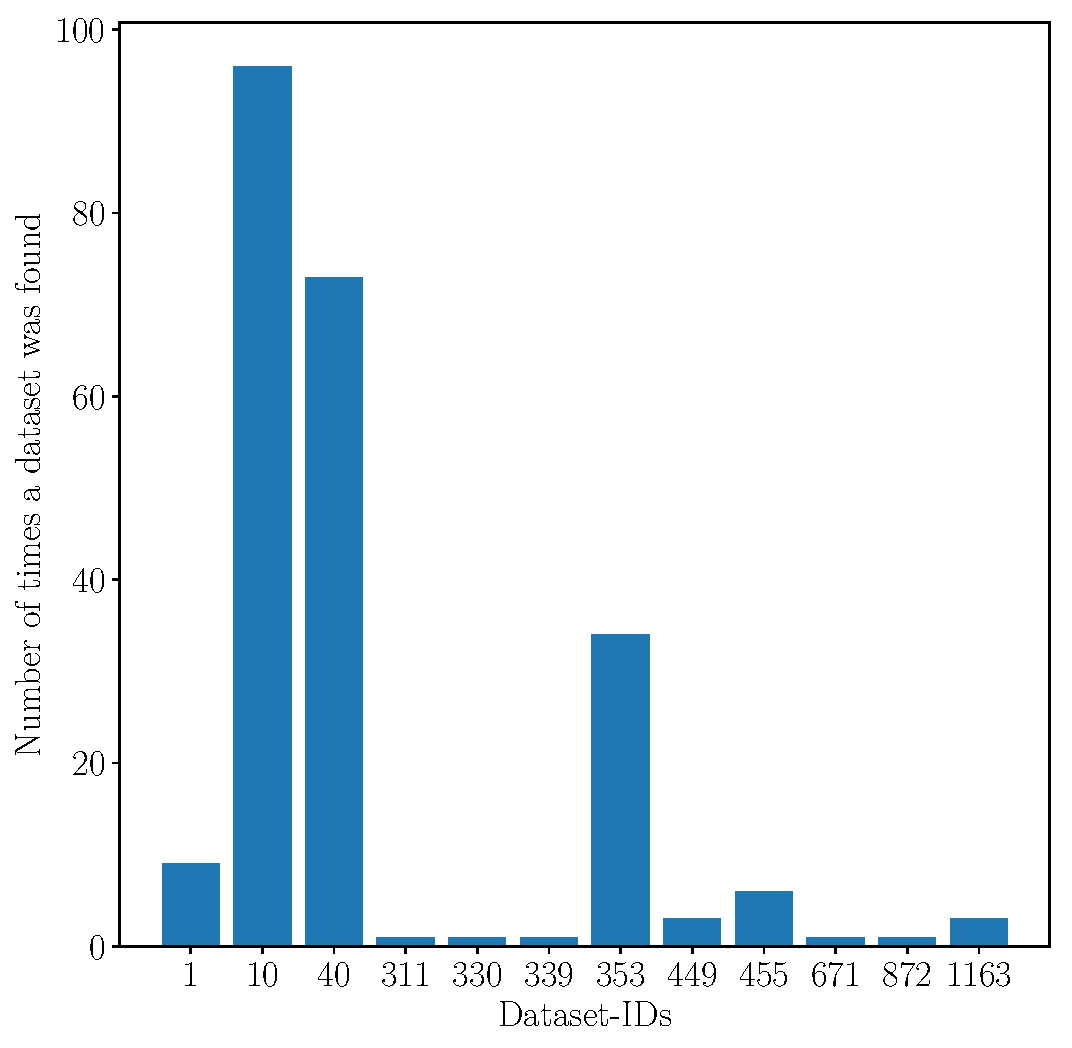
\includegraphics[scale=0.45]{images/freq.pdf}
    \caption{Frequency Distribution of Dataset Citations}
    \label{fig:graph}
\end{figure}
%\smallskip
\item \textbf{Rasa-based Dataset Detection:}
In our second approach, we trained an entity extraction model based on conditional random fields using Rasa NLU~\cite{DBLP:journals/corr/abs-1712-05181}. We particularly tested two configurations for training the CRF-based NER model. In Phase-1, the 2500 labeled publications from the training dataset were used for training the Rasa NLU\footnote{\url{https://rasa.com/docs/nlu}} model. Later in Phase-2, when the Phase-1 holdout corpus was released, we combined its 5000 labeled publications with the previously given 2500 labeled publications and then retrained the model again with these 7500 labeled publications. %The 7500 labeled publications from phase 1 corpus  (after preprocessing) are used for generating the training data for Rasa NLU. Specifications for model training are given below. 
\\
\textbf{Running the CRF-Model:} The trained model was run against the preprocessed data to detect dataset citations and mentions. Only the entities that had a confidence score greater than a certain threshold value (=0.72) were considered as dataset mentions. A dataset mention was considered as a citation only if it was found in the given Dataset Vocabulary and if it belonged to the research field of the article. %were considered as datasets and written to files. 
To check if a dataset belonged to the field of research, we found the cosine similarity of the terms in the ‘subjects’ field of the Dataset Vocabulary with the keywords, and identified the Research Field of the article. 
\smallskip
\item \textbf{Combining the two approaches:}
The output generated by the rasa-based approach was first checked for irrelevant citations before a union was performed to combine the results. %of both the approaches. 
This was done by checking if a given dataset\_id occured more than a threshold value (=1.20) multiplied by the median of the frequency distribution (same as the filtering process of the Simple Dataset Mention Search). %After filtering out such citations, the results of both the approaches were combined by taking a union  % two approaches above was checked for fake mentions before being written to the final output file data$_$set$_$citations.json, and data$_$set$_$mentions.json in data/output.  This is done by calculating the frequency of dataset mentions and removing mentions that occur more than a threshold$_$value * median of dataset$_$frequency.
\end{enumerate} 

Note that, the threshold values mentioned above were set after some experiments of trial and testing. For dataset extraction, the goal was to keep the number of false positives low while not compromising the true positives. %\todo[inline]{Not sure if you mean 'compromising with' or 'compromising'. The two mean different things. The first means altering with (using) the true positives and the second means altering the true positives themselves. ??} 
For research methods and fields, a manual evaluation (see the next section for details) was done to test if the results made sense with the articles.

\section{Evaluation}
We performed a quantitative evaluation for Dataset Extraction using the evaluation script provided by the competition organizers. This evaluation (see Table \ref{tab:dataset}) was carried out against the validation data, wherein we compared four different configurations. As can be inferred from the table, %\ref{tab:dataset}, 
there was only a slight increase in performance for the Rasa-based model, when the training samples were increased. However, combining it with the Simple Dataset Mention Search, increased the performance by \emph{19.42\%}. Interestingly, there was no improvement in performance in the combined approach even when the training samples for Rasa Model were increased. This might be because of the removal of frequently-occuring terms from the Rasa-generated output, based on the frequency distribution of dataset mentions as computed in the Simple Dataset Mention Search.  \\
%\todo[inline]{explain why no increase - no uniformity in labeled data}

%\todo[inline]{multirow heading for phase-1 and phase2 in table 1}

%\begin{center}
    %\myred{Quantitative Evaluation of Datasets against Validation data} \\
    %\bigskip
\begin{table}
    \captionsetup{justification=centering,margin=1.2cm}
    \caption{Quantitative Evaluation of Datasets against Validation Data. (The numbers inside brackets indicate training samples)} \label{tab:dataset}
    \begin{tabular}{ M{2.2cm} | M{2.3cm} |  M{2.2cm} M{2.2cm} M{2.2cm} }
        \toprule
        \multirow{2}{*}{} & \multicolumn{1}{c|}{\textbf{Phase-1}} & %
        \multicolumn{3}{c}{\textbf{Phase-2}} \\
        \cmidrule{2-5}
        \textbf{Metrics}& \textbf{Rasa-based Approach} (2500)  & \textbf{Rasa-based Approach} (7500) & \textbf{Combined Approach} (2500)  & \textbf{Combined Approach} (7500) \\ \hline
        \textbf{Precision} & 0.382 & 0.388 & \textbf{0.456}  & \textbf{0.456} \\
        \textbf{Recall} & 0.26 & 0.26 & \textbf{0.31} & \textbf{0.31} \\
        \textbf{F1} & 0.309 & 0.311 & \textbf{0.369} & \textbf{0.369} \\
        \bottomrule
    \end{tabular} 
\end{table} 
%\end{center}
%\smallskip

For Research Fields and Methods, we carried out a qualitative evaluation against 10 randomly selected articles from Phase-1 holdout corpus. Tables \ref{tab:field} and \ref{tab:method} depict a comparison between the predicted fields and methods in Phase-1 and Phase-2. In general, our models returned a more granular output in the second phase, solely because of the modifications we made in the vocabularies. 


%\myblue{Evaluation against Phase-1 holdout} \\
%\bigskip
\begin{table}
\caption{Evaluation of Research Fields against Phase-1 holdout} \label{tab:field}
\begin{tabular}{C{1cm} C{4.5cm} C{3cm} C{3.5cm}} \hline
    \textbf{pub\textunderscore id} & \textbf{Keywords} & \textbf{Phase-1}  & \textbf{Phase-2} \\ \hline
     10328 & Cycling for transport, leisure and sport cyclists & Health evaluation & \textbf{Public health and health promotion} \\ \hline
     7270 & Older adult drug users, harm reduction & Health Education & \textbf{Correctional health care} \\ \hline
    6053 & Economic conditions - crime relationship, homicide & Homicide & \textbf{Gangs and crime} \\ \hline
\end{tabular}
\end{table}

\begin{table}
\caption{Evaluation of Research Methods against Phase-1 holdout} \label{tab:method}
\begin{tabular}{C{1cm} C{4.5cm} C{3cm} C{3.5cm}} \hline
    \textbf{pub\textunderscore id} & \textbf{Keywords} & \textbf{Phase-1}  & \textbf{Phase-2} \\ \hline
     10328 & Thematic content analysis & Thematic analysis & \textbf{Sidak correction} \\ \hline
     7270 & Interviews conducted face to face, finding systematic patterns or relationships among categories identified by reading the interview transcript & Qualitative interviewing & \textbf{Sampling design} \\ \hline
    6053 & Autoregressive integrated moving average (ARIMA) time-series model & Methodological pluralism & \textbf{Multivariate statistics} \\  \hline
\end{tabular}
\end{table}

\section{Discussion}
%\todo[inline]{challenges encountered}
Throughout the course of this competition, we encountered several challenges and limitations in all the three stages of the pipeline. In the preprocessing step, the appropriate extraction of text from PDFs turned out to be rather challenging. This was especially due to the varied formats of the publications, which made the extraction of specific sections---that contained all data relevant to our work---demanding. As mentioned before, if there was no explicit mention of the key-terms like \texttt{Abstract, Keywords, Introduction, Methodology/Data, Summary, Conclusion} in the text, then the content was saved as `reduced\_content' after applying all other preprocessing steps and filtering out any irrelevant data. \\

Our experiments suggest that the labeled publications we received for dataset detection were not uniform in the dataset mentions provided, which made it difficult to train an entity extraction model even with an increased number of training samples. Hence, there was only a slight improvement in performance when the Rasa-model was trained with 7500 publications instead of 2500. This was also why we combined the Rasa-based approach with the Simple Dataset Mention Search, so that at least the datasets that were present in the vocabulary didn't get missed. 

Regarding the fields and methods, vocabularies played an immense role in %the process of 
their identification. The vocabularies that were provided by the SAGE publications contained some terms that were either polysemous or very high-level and therefore, were picked up by our model very often. Hence, for research methods, we created our own vocabulary containing all the relevant statistical methods, and for fields, we introduced a blacklist of irrelevant terms and looked it up each time, before writing the result to the output file. Since the focus was on more granulated results, we tried to look for open ontologies for Social Science Fields and Methods and unfortunately, could not find any. It is worth mentioning that since our approach for Fields and Methods identification relied heavily upon vocabularies, it could not find any new methods or fields from the publications. 

\section{Future Agenda}
The data provided to us in the competition displayed a cornucopia of inconsistencies even after human processing. We hence propose that machine-aided methods for computing correct and complete structured representation of publications are of central importance for scientific research. Previous works on never-ending learning have shown how humans and extraction algorithms can work together to achieve high-precision and high-recall knowledge extraction from unstructured sources. In our future work, we hence aim to 
%While building models to extract information from such data, we gained insights into how we could benefit from having an even greater amount of publications. With the number of publications growing every year and new innovations making their way in, it is imperative to have a system that could update itself with the desired information and hence, record the metadata of ongoing research. To this end, 
populate \textbf{scientific knowledge graphs} based on never-ending learning. The methodology we plan to develop will be domain-independent and rely on active learning to classify, extract, link and publish scientific research artifacts extracted from open-access papers.  % comprising all the scientific domains and not just the field of social sciences. 
The resulting graphs will
\begin{itemize}
    %\item follow the concept of never-ending learning.
    \item rely on advanced distributed storage for RDF to scale to the large number of publications available;
    \item be self-feeding, i.e., crawl the web for potentially relevant content and make this content available for processing;
    \item be self-repairing, i.e., be able to update previous extraction results based on insights gathered from new content;
    \item be weakly supervised by humans, who would assist in correcting wrong hypotheses;
    \item provide standardized access via W3C Standards such as SPARQL.
\end{itemize}

Having such knowledge graphs would make it easier for the researchers (both young and veteran) to easily follow along with their domain of fast-paced research and eliminate the need to manually update the domain-specific ontologies for fields, methods and other metadata as new research innovations come up. 

%\end{multicols}

\bibliographystyle{plain}
\bibliography{references} 
% \todo[inline]{ First, the judges will take a random set of publications and score precision and recall based on that set.   Second, as our technical judges suggested, since this phase of the competition is to be much more collaborative, you to help us design the evaluation.  As such, we ask that your team supply us with a short, one-page description of your planned approach for working on the Phase II challenge. We want you to tell us (broadly) your approach – your secret sauce – and tell us how would you like to be evaluated.  }
% \todo[inline]{@Rricha/Nikit: Combine text below with stuff from here, i.e. what we actually used: Preprocessing:
% Handling of words that get split by hyphens
% The identification and extraction of certain sections (e.g., title, abstract, methodology, etc.)
% Removal of non-text objects (e.g., graphs, equations, etc.) 

% Extraction of dataset mentions
% (Datasets) René Pattern-based approaches on the dependency trees of sentences [2] using handwritten as well as learned rules
% (Datasets) Daniel does RASA NLU based NER
% Merging of the two approach

% Research fields and methods
% Rricha: prepare a file with all NNP for all docs
% Consider preprocessing from above
% Compute parse tree for all sentences in D
% Gather all NPs $noun_1 … noun_m$
% Including sub-phrases of longer phrases
% Micha/Nikit: Vectorize dictionaries we received where every label comprises a set of words ${w_1 … w_n}$, create $v(w_1 … w_n) = \sum\limits_{i=1}^n v(w_i) $
% Where $v(w_i)$ is the vector of word$w_i$ in the embedding space
% Micha/Nikit:  Given a document D
% Compute $cos(v(noun_i), v(w_dict_j))$ for all NPs in $D$ and all $w_dict$ in the dictionary
% Select highest score $w_dict$ as field/method
% }

% We preprocess the plain text of the documents. In detail, this includes the handling of words that get split by hyphens, the identification and extraction of certain sections (e.g., title, abstract, methodology, etc.), as well as the removal of non-text objects (e.g., graphs, equations, etc.) from these sections.

% For the extraction of the research field, method and dataset mentions, we will follow two different pattern-based approaches on sentences [1] and on the dependency trees of sentences [2] using handwritten as well as learned rules. Since authors generally include the main contribution of the paper in the title, we would use titles (given in the article\_metadata) and abstracts to find the research fields and research methods (and also the dataset, if possible). In addition to this, we would also apply these approaches to the methodology and data section for the identification of research methods and dataset mentions.  
% While exploring the publications data, we observed that a dataset mention is always followed or preceded by an explicit mention of terms like ‘data’, ‘dataset’ or the likes. These terms together with the functional keywords like ‘use’, ‘utilize’, ‘gather’, etc. would act as a seed-set for our pattern matching approach for identifying datasets. If the identified dataset is present in the given dataset vocabulary, we will find all the dataset mentions using the same pattern matching approaches on the remaining sections of the paper (results, conclusions, discussions, summary, etc) for generating the publication-dataset relation file, else we will add it to the dataset mention output file. 

% After extracting the mentions, we will disambiguate them using AGDISTIS [3]. Therefore, we will create a knowledge base containing the given research fields, methods and datasets as RDF resources with connections gathered from the training data. AGDISTIS will use the trigram similarity between the mentions and the known research fields, methods and datasets as well as their connections to each other to either link the mentions to a known resource or create a new resource.

% For our experiments, we will use a Linux-based (Ubuntu 18.04.1 LTS) system with 8 Intel Xeon CPU E5-2620 v4 @ 2.1GHz cores (=16 virtual cores) and 128 GB RAM. 


% Link to Github?: https://github.com/dice-group/rich-context-competition
\end{document}
